\documentclass[a4paper]{article}
\usepackage[utf8]{inputenc}
\usepackage[english, bulgarian]{babel}
\usepackage{sectsty}
\usepackage{pdfpages}
\usepackage{titlesec}
\usepackage{titletoc}
\usepackage{hyperref}
\usepackage[all]{hypcap}
\usepackage{graphicx}
\usepackage{nameref}
\usepackage[symbol]{footmisc}
\usepackage{fixfoot}
\usepackage{xspace}

% Times New Roman 12pt
\documentclass[12pt]{book}
\usepackage{mathptmx}

% Equivalent of 1.5 in Word
\onehalfspacing

\graphicspath{ {./images/} }
\hypersetup{
colorlinks=false
}

\usepackage{etoolbox}% provides \patchcmd
\makeatletter
\patchcmd\@fixed@footnote
  {\protected@xdef\@thefnmark{\csname @#1@fftn@footnote\endcsname}}% search
  {\protected@xdef\@thefnmark{%
     \expandafter\@fnsymbol\csname @#1@fftn@footnote\endcsname}}% replace
  {}{}% success/failure
\makeatother

\DeclareFixedFootnote\underdev{в процес на разработка}
\DeclareFixedFootnote\unsure{не е сигурно}

\titleformat{\section}
   {\Huge\bfseries\centering}% format
   {}% label
   {}% sep
   {}% before code
   [{\titlerule}]% after code
 
 \titleformat{\subsection}
   {\LARGE\bfseries\centering}% format
   {}% label
   {}% sep
   {}
   
\titleformat{\subsubsection}
   {\large\bfseries\centering}% format
   {}% label
   {}% sep
   {}
   
   
 \titlespacing*{\section}
   {0pt}% left
   {0pt}% before sep
   {0.7cm}% after sep
   
\titlespacing*{\subsection}
   {0pt}% left
   {0.5cm}% before sep
   {0.5cm}% after sep
   
\begin{document}

\allsectionsfont{\centering}
\centering
\title{LuncherBox - Интерактивно Меню}
\author{Симо Александров и Любо Любчев}
\date{Февруари 2019}
\centering
\maketitle

%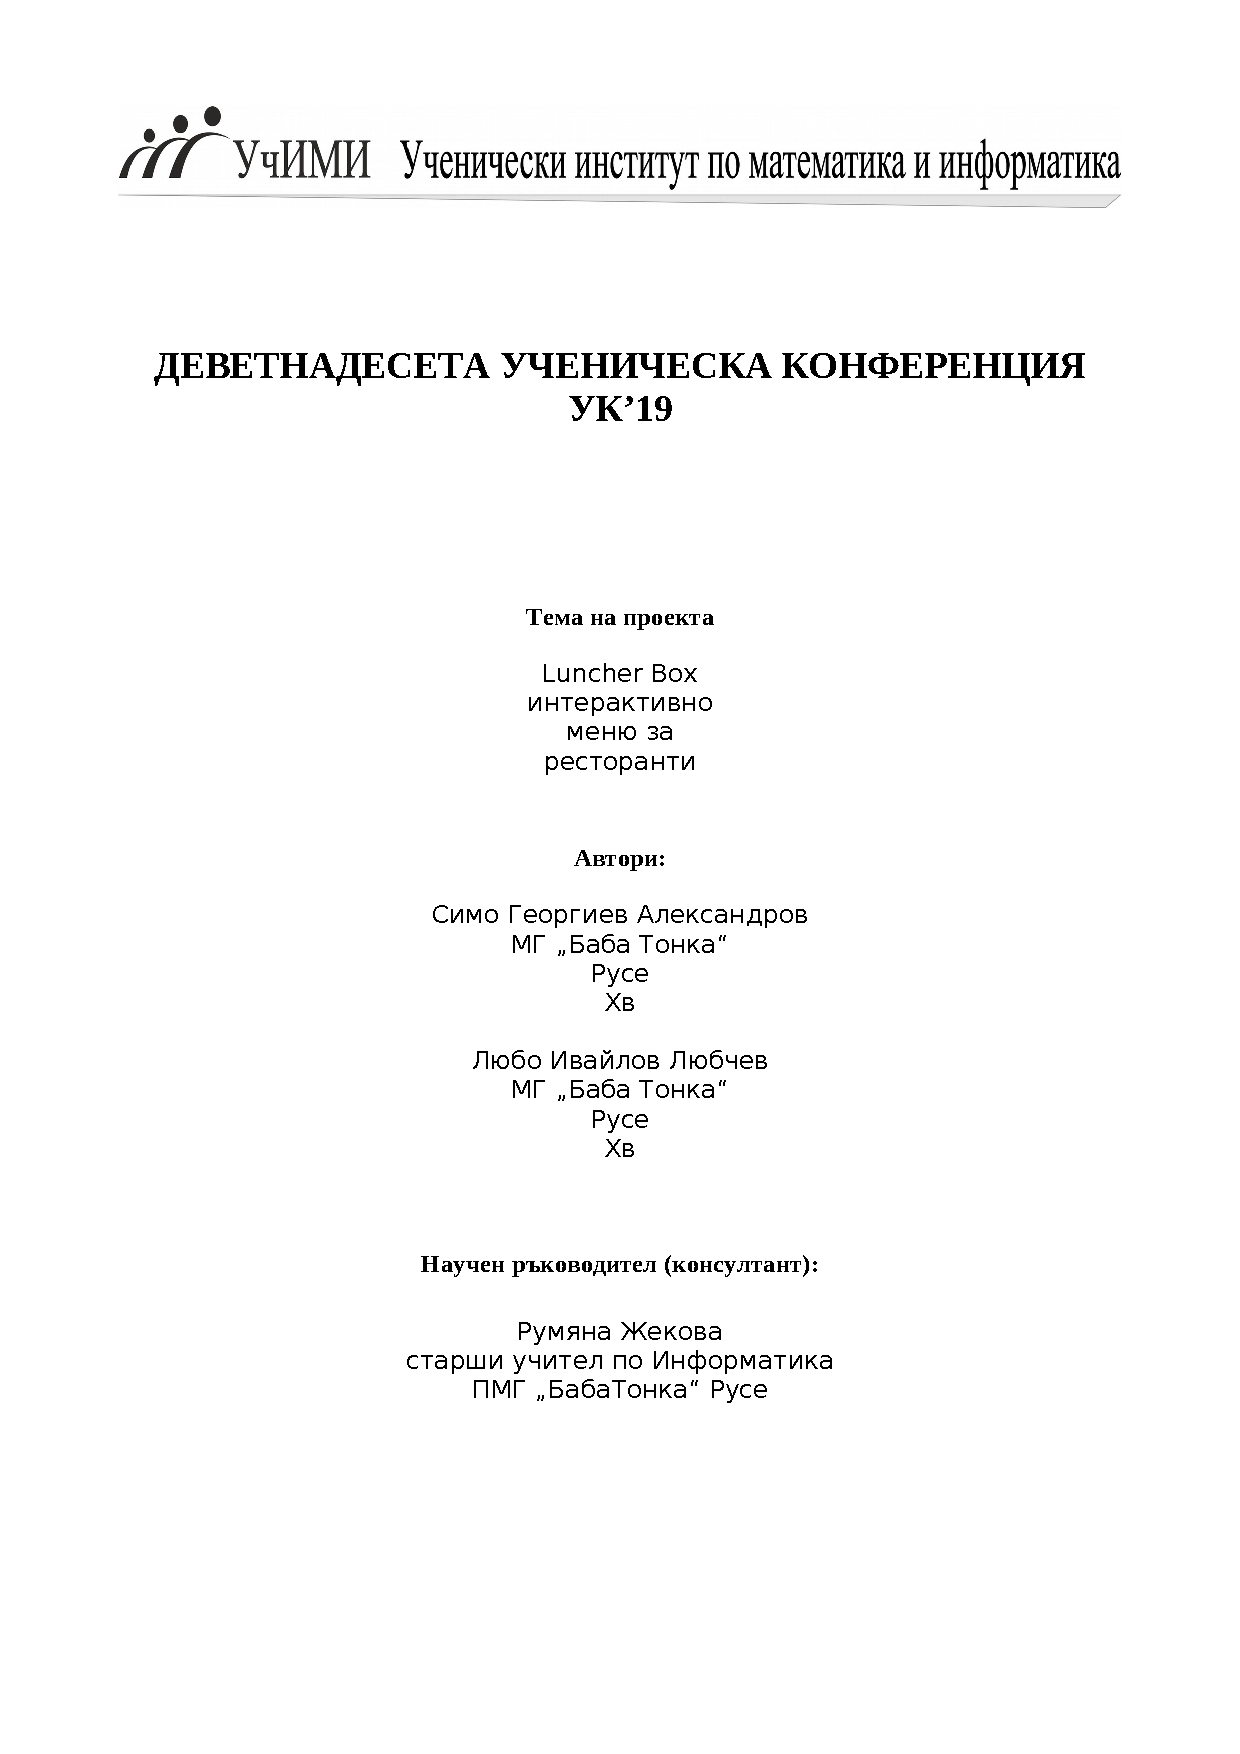
\includepdf[pages=-]{header.pdf}

\newpage

\begin{abstract}
\textbf{Luncher Box - Интерактивно Меню} е уеб приложение, което цели поръчването на храна от клиенти в ресторанти да става по-бързо. 
Освен доволни клиенти, собствениците на заведението ще спестяват пари, чрез свеждане на нуждата от сервитьори до минимум. 

Проектът е с приложен характер, все още е в процес на разработка и е от сферата по информатика и информационни технологии. Идеята е измислена от Любо Любчев, а е реализирана от двамата автори. 

Клиентите на ресторанта ще осъществяват поръчките си, чрез ``Luncher Box'', който ще изпрати заявката към кухнята, където тя ще бъде приета и обработена отново през приложението.
\end{abstract}
\begin{figure}[h]
\centering
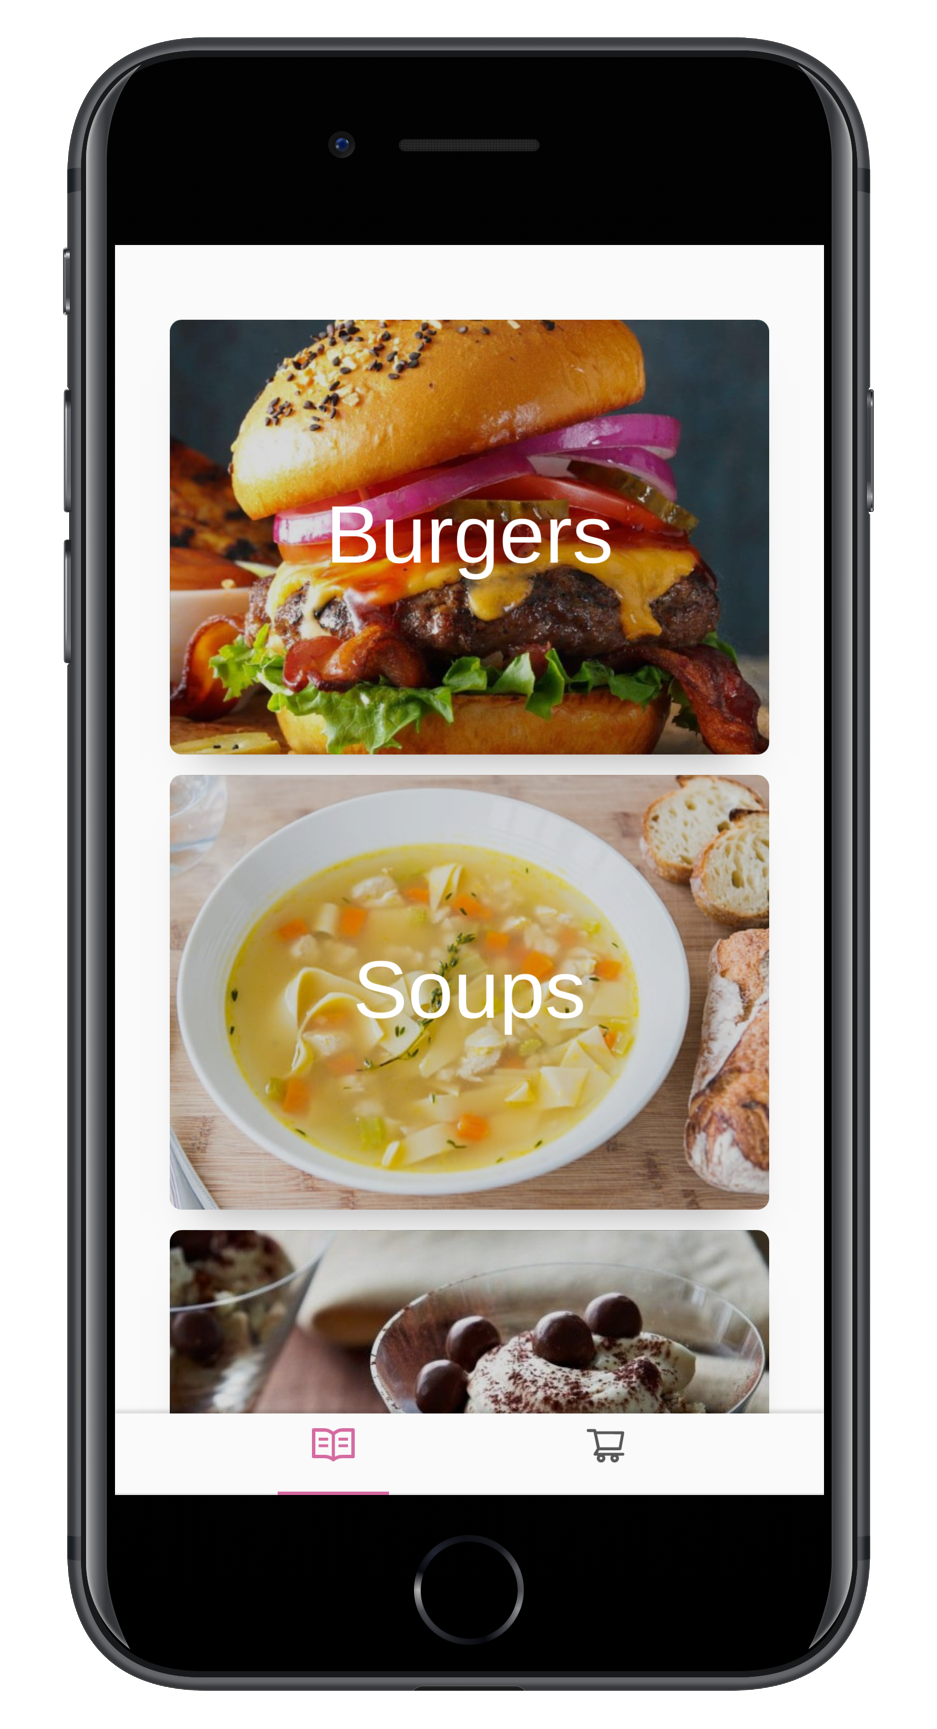
\includegraphics[height=9cm]{{images/iphone.png}}
\end{figure}

\selectlanguage{english}
\begin{abstract}
\textbf{Luncher Box - Interactive Menu} is a web app which aims making placing orders by clients in restaurants a much faster task.

Other than the satisfied customers, the restaurant owners will save money by lowering the required amount of waiters to a minimum. 

The project has applicational nature, it is still under development and belongs to the IT field. The idea was conceived by Lyubo Lyubchev and was realised by both of the authors.

The clients of the restaurant will place orders through ``Luncher Box'', which will send the request to the kitchen, where it will be processed through the app.

\end{abstract}
\selectlanguage{bulgarian}
\newpage
\tableofcontents
\newpage

\section{Увод}
\begin{Large}

Много често клиентите на ресторантите чакат прекалено дълго само за да направят поръчка - изискват се доста сервитьори, за да обслужат всички, от това следва спад на общата ефективност на заведението.

С тази разработка целим намаляването или премахването на времето, нужно за чакане преди да се приемат и изпълняват поръчки в заведения. Това ще допринесе до по-висока ефективност на ресторантите, тъй като се намаля нужния брой сервитьори, а така ще се намалят и разходите на ресторанта. Целим се в създаването на решение, което не изисква покупката на отделно устройство за всяка маса.

За да постигнем горепосочените цели, сме си поставили малко, но за нас предизвикателни задачи, а именно следните:

\begin{itemize}
\item Планиране на архитектура и подбор на правилните технологии;
\item Разработка на backend сървър;
\item Оформяне на красив и интуитивен графичен интерфейс;
\item Създаване на цялостно функциониращо уеб приложение, което ще работи само в локалната мрежа на ресторанта;
\item Рекламиране на продукта;
\item Разпространяване на продукта.
\end{itemize}

В следващите глави ще задълбочим как приложението ще работи и как ще решим тези задачи.

\newpage

\section{Галерия}
\begin{figure}[h]
\centering
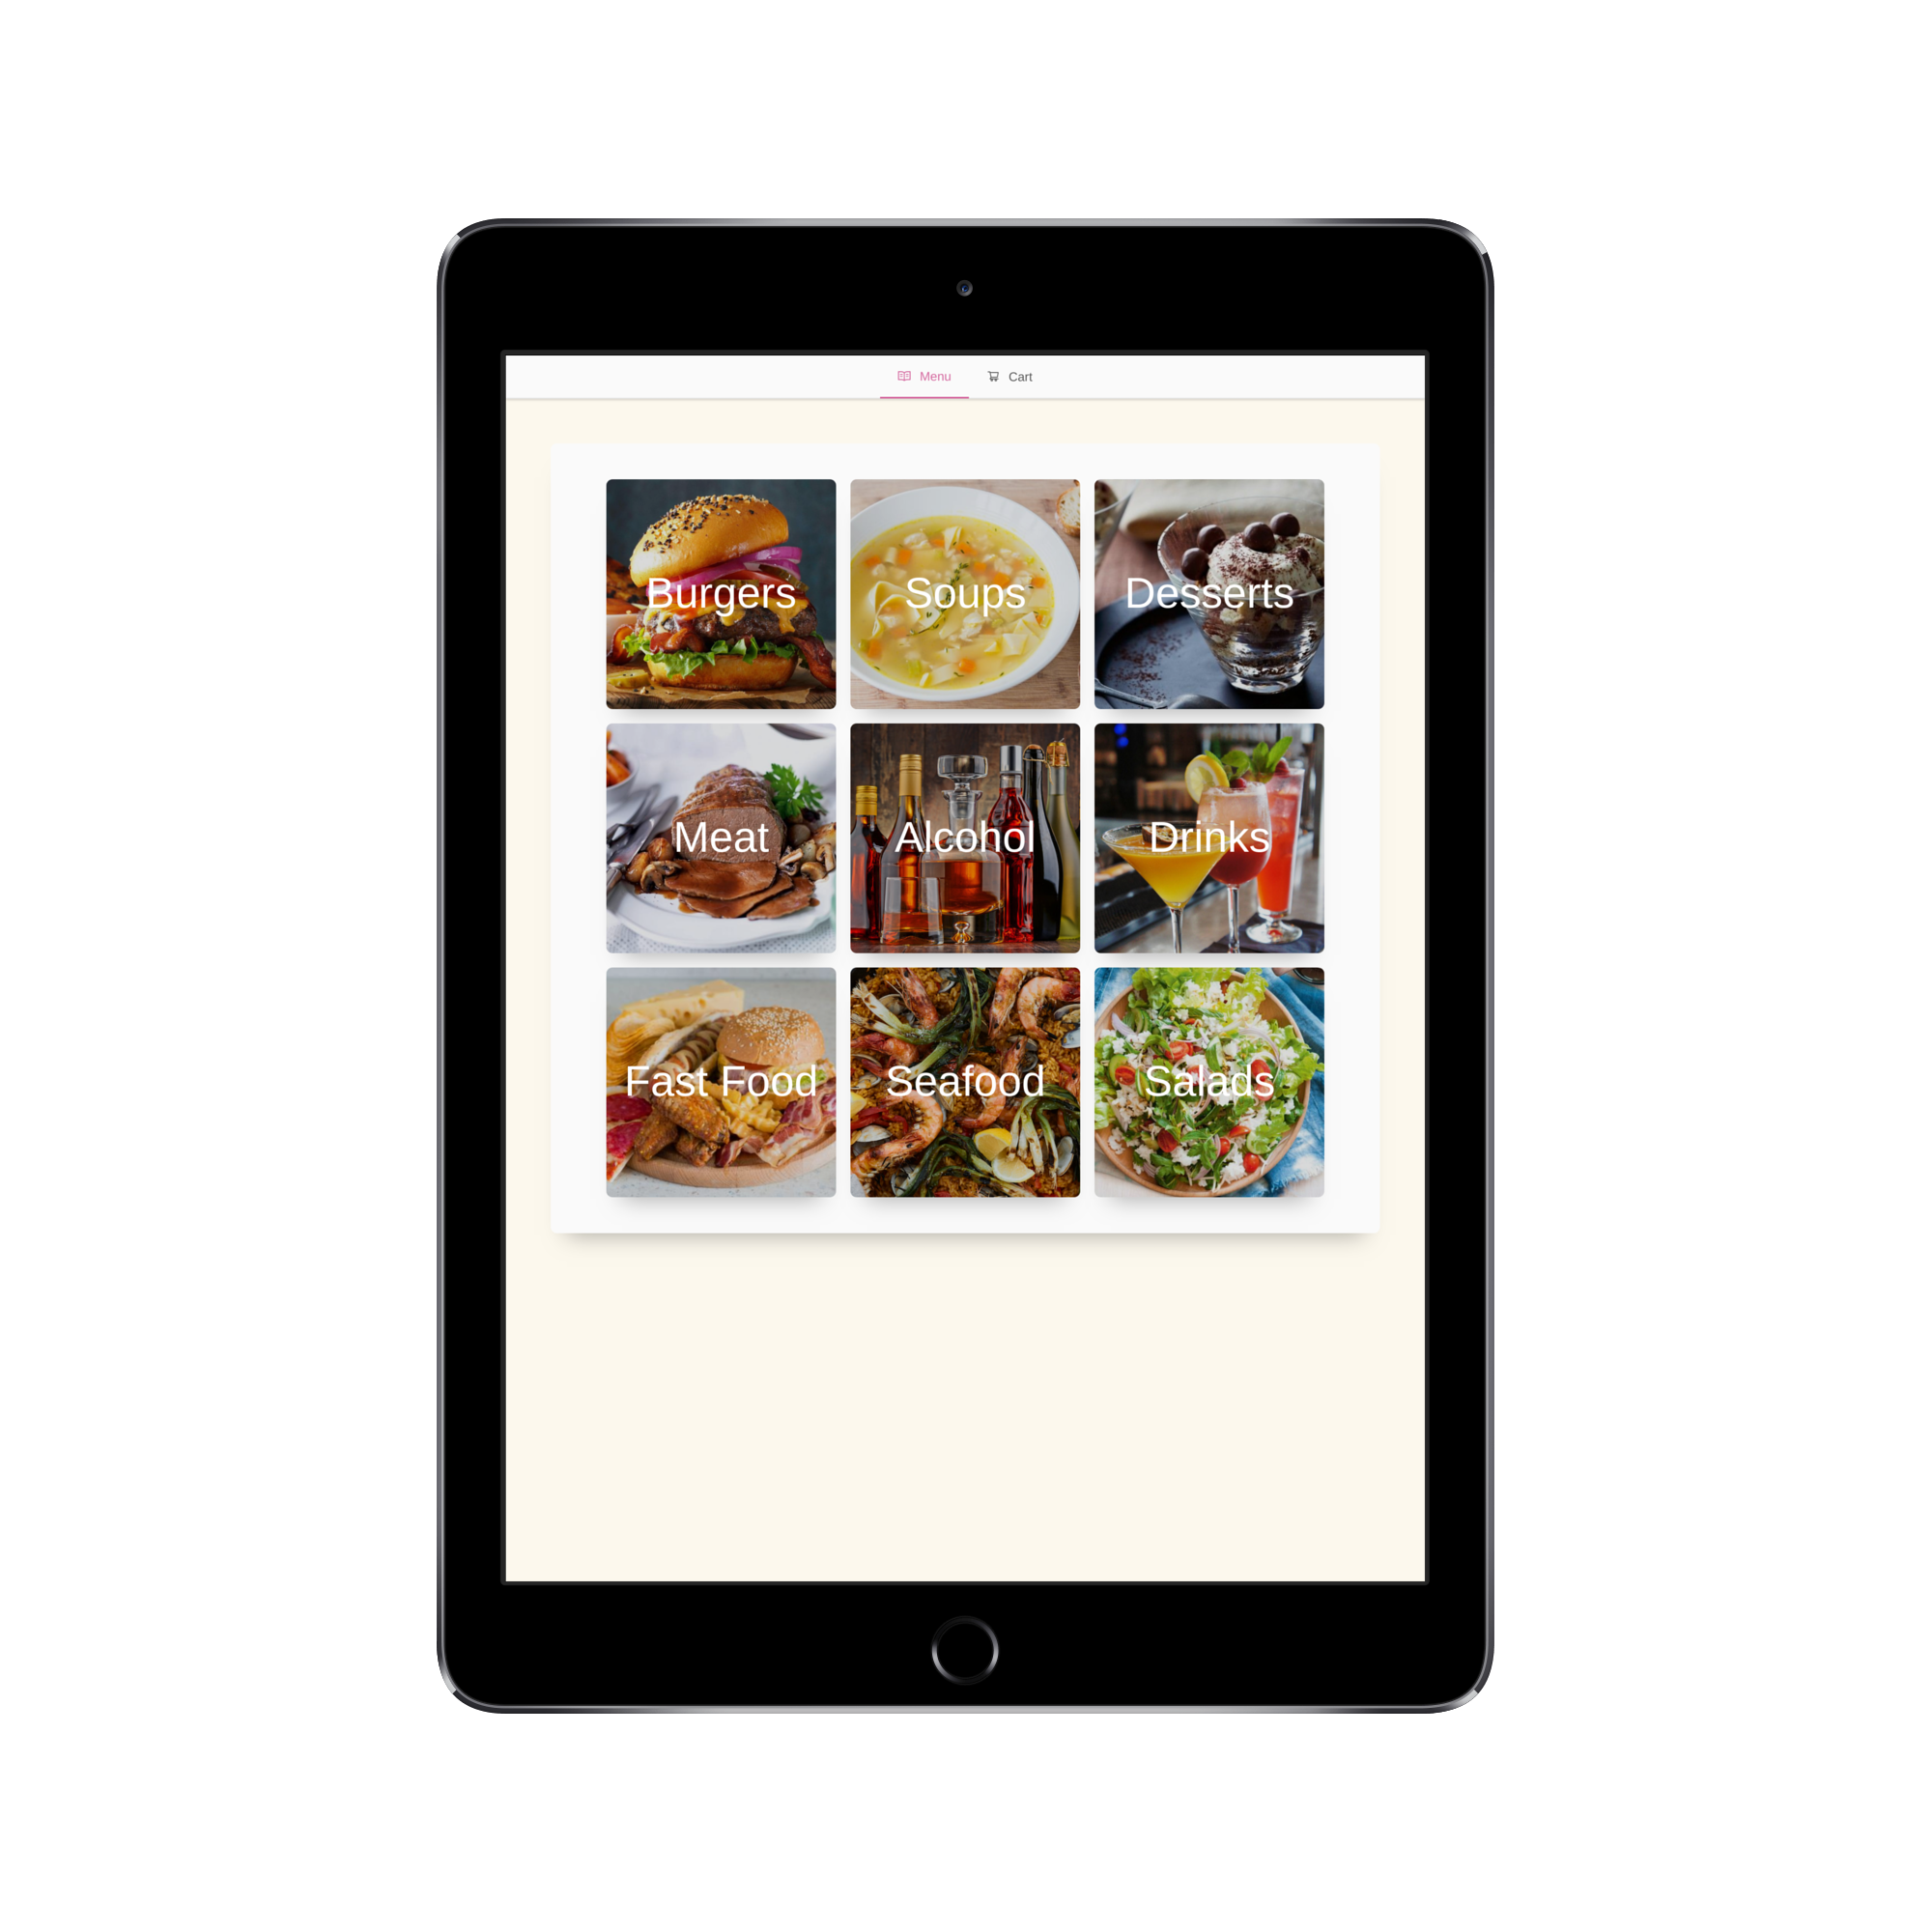
\includegraphics[height=8.5cm]{{images/ipad.png}}
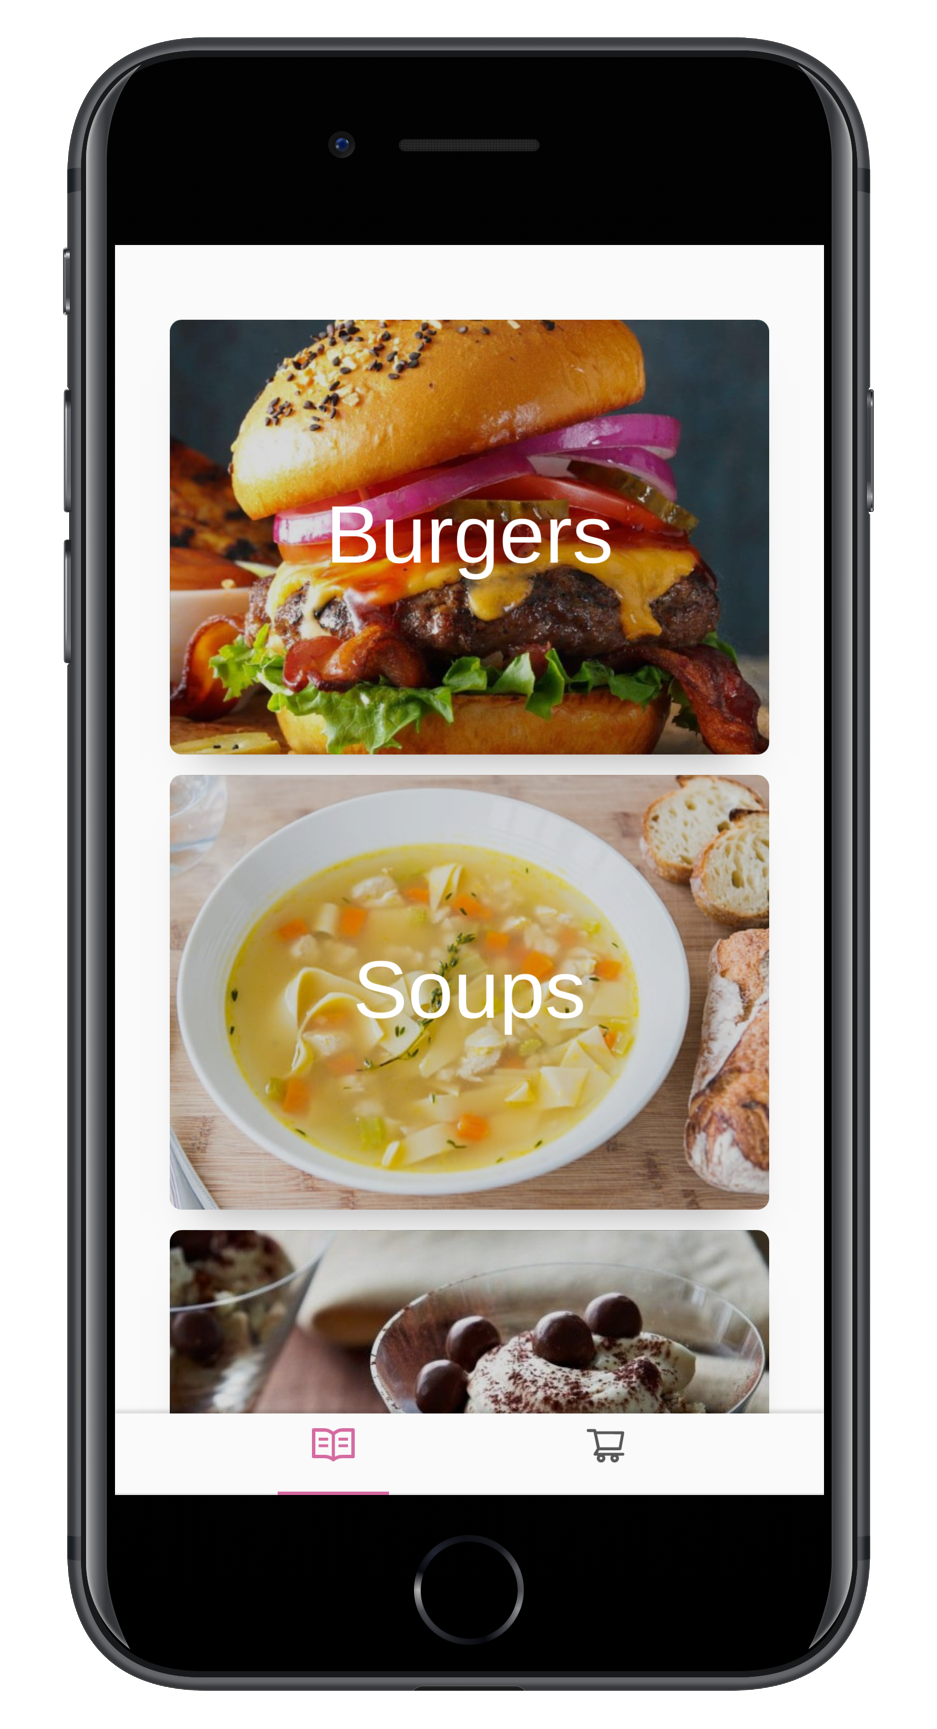
\includegraphics[height=7cm]{{images/iphone.png}}
\caption{Преглед на различни устройства}
\end{figure}
\newpage

\section{Функции}


Приложението предоставя следните функции:

\begin{itemize}
\item Лесен, красив, бърз и интуитивен интерфейс за всички резолюции;
\item Административен панел;
\item Потребителски панел;
\item Директен достъп до менюто на ресторанта;
\item Масово импорт-ване и експорт-ване на продукти в различни формати като - \textbf{JSON}, \textbf{YAML}, \textbf{CSV} или \textbf{XML};\underdev
\item Правене и отказ на поръчка към кухнята без нужда от регистрация;
\item Статус на поръчката;
\item Плащане чрез кредитна/дебитна карта, в брой или криптовалута;\underdev
\item Автоматично запазване на продуктите в количката.
\end{itemize}
\newpage
\setcounter{footnote}{0}
\section{Как работи?}


На всяко заведение ще му бъде предоставено устройство (например Raspberry Pi), на което приложението ще се хоства на локалната мрежа. По този начин, приложението ще може да се използва само в обсега на ресторанта. При поставянето на поръчка, клиентът ще бъде помолен да извърши плащане или чрез кредитна/дебитна карта, в брой или с криптовалута, предотвратявайки експлоатация от външни клиенти. 

\subsection{Потребителски панел}

Използването на приложението ще бъде лесна задача. Клиентът ще трябва да се свърже за интернет мрежата на ресторанта, използвайки собственото си мобилно устройство. След осъществената връзка, потребителят ще достъпи менюто през browser-а си. Вследствие на това клиентът може да избере продукти, които може да добави чрез ``\textbf{+}'' бутона. (фиг. \ref{fig:product})

\begin{figure}[h]
\centering
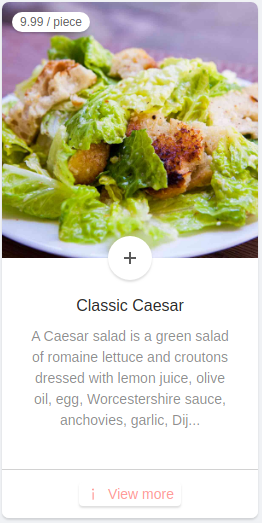
\includegraphics[height=5.2cm]{{images/product.png}}
\caption{Продукт\label{fig:product}}
\end{figure}

След добавянето, продуктът се добавя в количка, която държи предишно добавените продукти. 
\newpage
Когато клиентът счита, че е готов за поръчка, той може да я осъществи в таб-а на количката. (фиг. \ref{fig:cart})

\begin{figure}[h]
\centering
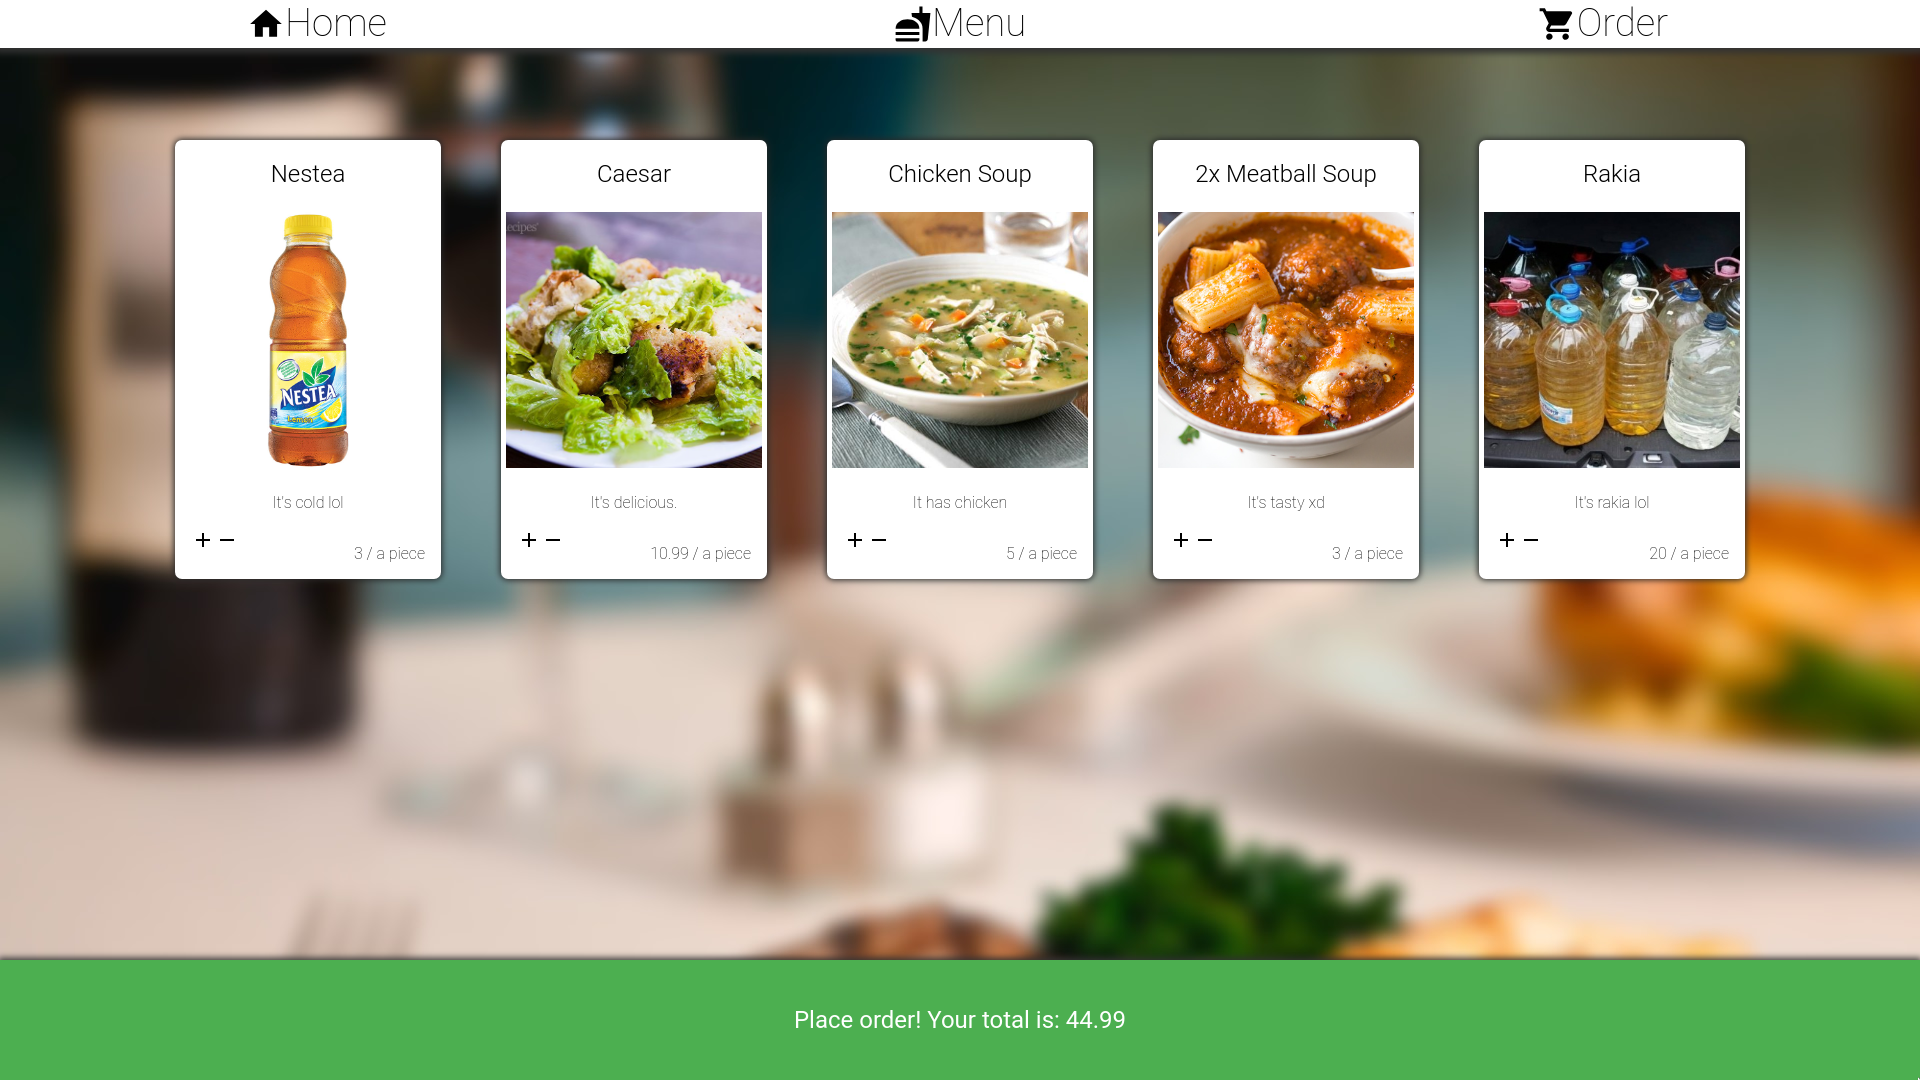
\includegraphics[width=\textwidth]{{images/cart.png}}
\caption{Количка\label{fig:cart}}
\end{figure}

Тук потребителя може да завърши неговата поръчка с натискането на зеления бутон.
Вследствие на това, клиента трябва да избере метод на плащане и да заплати.

\subsection{Административен панел}


При успешно изпратена поръчка от клиента, тя ще се появи в административния панел. Там готвачите мигновено ще виждат новите поръчки и ще могат да уведомят клиентите кога ще е готова директно през приложението. Всеки готвач и сервитьор ще има собствени потребителски профили, чрез които ще влизат в административният панел. (фиг. \ref{fig:admin-dashboard})

Друга функция е лесното добавяне, обновяване и премахване на продукти и категории. (фиг. \ref{fig:add-product})

\begin{figure}[h]
\centering
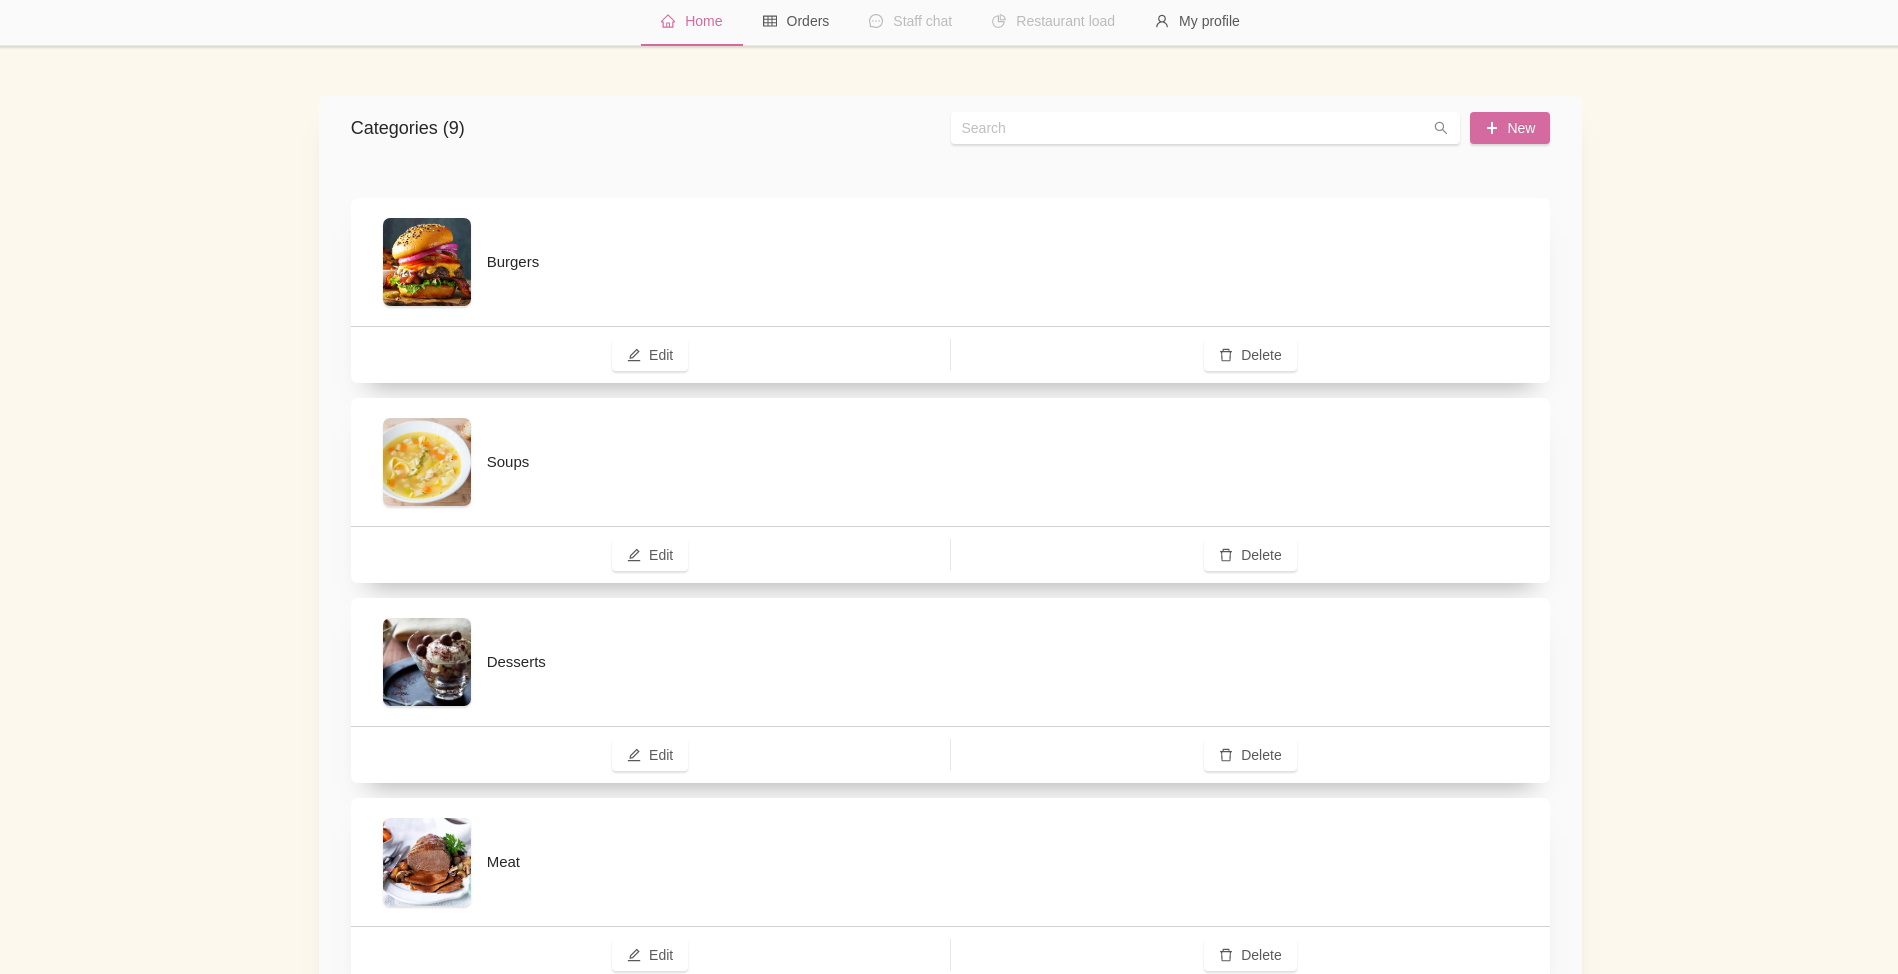
\includegraphics[width=\textwidth]{{images/admin.png}}
\caption{Административен панел\label{fig:admin-dashboard}}
\end{figure}
\begin{figure}[h]
\centering
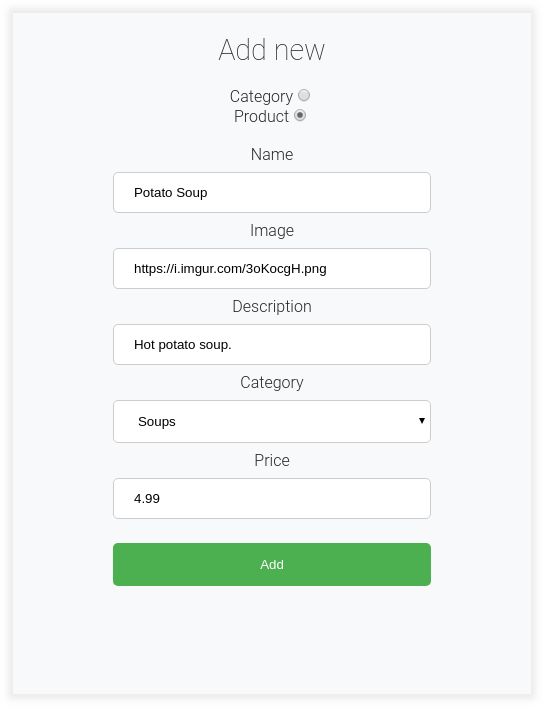
\includegraphics[height=10cm]{{images/add-product.png}}
\caption{Добавяне на продукт\label{fig:add-product}}
\end{figure}


\clearpage
\section{Технологии\label{tech}}




Като език на програмиране използвахме \textbf{TypeScript}, тъй като, може да се използва за frontend и за backend, е cross-platform, е statically typed и синтаксиса не е сложен за разбиране.


\subsection{Backend} 

\subsubsection{node.js}

Избрахме \textbf{node.js} защото е високоскоростен, високопроизводителен, щадящ ресурси, ефикасно комуникиращ в реално време, гъвкав и лесен за разработване environment на \textbf{TypeScript / JavaScript}. 

\subsubsection{express.js}

За HTTP сървър подходихме с \textbf{express.js}, тъй като тя ни предоставя абстракцията за създаване REST API, вместо да задълбаваме подробно в прости неща като CRUD операциите.

\subsubsection{passport.js}

\textbf{Passport.js} избрахме за създаване на профили както и за управлението на автентикация.

\subsubsection{nodemailer}

\textbf{Nodemailer} бе използван за изпращане на e-mail-и за потвърждаване на потребители.

\subsubsection{TypeORM и MySQL}

Решихме да имплементираме \textbf{TypeORM} за ORM, а \textbf{MySQL} за база от данни, тъй като e скалираща база от данни и ще е устойчива дори и в най-натоварените ресторанти.

\subsubsection{ioredis и Redis}

Ползвахме \textbf{ioredis} клиента за \textbf{redis} за session store, кеширане на \textbf{MySQL} query-та и държене на поръчки.

\subsubsection{socket.io}

За realtime връзката между backend и frontend използвахме \textbf{socket.io}, поради леснотата му на използване.

\subsection{Frontend}

\subsubsection{react.js}

За да създадем хубав и гъвкав интерфейс, заедно с reusable компоненти използвахме \textbf{react.js} - библиотека, създадена от Facebook.

\subsubsection{next.js}

За да създадем SPA и PWA използвахме \textbf{next.js} - библиотека, която предоставя SSR.

\subsubsection{node.js}

Тъй като библиотеката \textbf{react.js} е зависима от \textbf{node.js}, се наложи да го използваме и за frontend-а.

\subsubsection{socket.io}

За приемането и изпращане на поръчки използвахме \textbf{socket.io}.

\subsection{Архитектура}

Визуализирайки архитектурата на ``Luncher Box'', тя ще изглежда по следния начин (фиг. \ref{fig:arch}):

\begin{figure}[h]
\centering
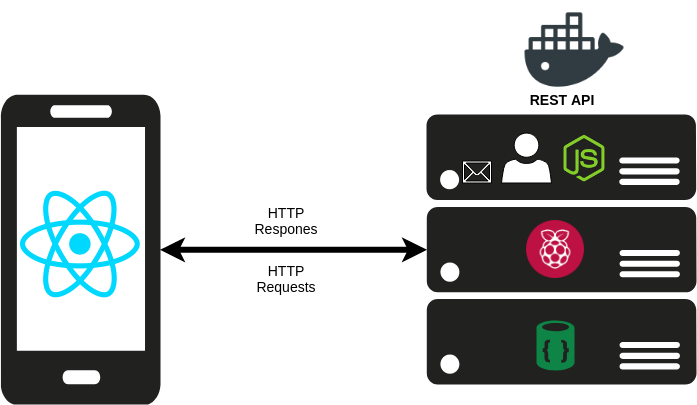
\includegraphics[width=\textwidth]{{images/arch.png}}
\caption{Архитектура\label{fig:arch}}
\end{figure}
\newpage
\section{Етапи на развитие}

\subsection{Избор на тема}

Двама от авторите сме забелязвали дългото чакане по заведенията само за да бъде взета поръчката. В продължение на 30 мин. размишляване по време на чакането в едно от заведенията, започнахме да се чудим как да оптимизираме целия процес със знанията, които имаме. Хрумна ни, какво можем да направим по въпроса - да създадем интерактивно меню. Чрез него клиентите ще могат директно да изпращат поръчки към кухнята или бара на заведението.

\subsection{Проучване}

Бяха проучени няколко подобни решения, но се оказа, че имат следните изисквания:
\begin{itemize}
\item Регистрация за правене на поръчки;
\item Отделно хардуерно устройство на всяка маса.
\end{itemize}

При изискването на отделно хардуерно устройство за всеки клиент или маса, се изисква висок начален капитал.

Убедихме се, че има неща, които могат да се подобрят в другите решения, спестявайки доста ресурси и време както на клиентите - липсата от нужда за регистрация, а на собствениците нуждата от купуването на устройства.

\subsection{Избиране на технологии и архитектура}

През този етап ни минаха доста идеи относно подхода ни с технологиите, като се спряхме на вече гореспоменатите. (Виж сек. \ref{tech} - \nameref{tech})

\subsection{Изработване}

По време на различни хакатони, работихме върху приложението.

Създадохме прост REST API, чрез който извършвахме прости CRUD операции.

Създадохме базов прототип на дизайна в \textbf{Figma}, по който си структурирахме разработката на frontend–а.

Свързахме frontend-а с backend-а чрез HTTP заявки и отговори.

\newpage

\section{Конкуренция}

В процеса на създаване на приложението, бяха прегледани няколко решения, които имаха недостатъци, които ние разрешихме. 

Например голяма част от тях изискват покупката на отделни устройства на всяка маса - таблет, специален екран вграден в масата или други, също така почти всички имаха ужасен интерфейс. 

За разлика от конкуренцията, ние се целим да решим тези проблеми. Основния от тях е нуждата от покупката на отделни устройства за всяка маса. Ние разрешаваме този проблем като създадохме уеб приложение, което може да използва от всякакъв вид устройства, стига да могат да отварят уеб страници. Самият сървър ще бъде хостван на само едно устройство, а като алтернатива може да бъде използван компютъра на заведението, ако има такъв.



\newpage 

\section{Заключение}

\textbf{Luncher Box - Интерактивно Меню} ще спести много време на клиентите на заведения, като им предостави онлайн интерактивно меню с лесен за използване интерфейс.  Те ще могат да го отворят през browser-ите си и да направят поръчка без да чакат, поради липсата на нужда от сервитьор. А собствениците на ресторанта ще могат да спестят пари от намаляването на служители.

Въпреки предизвикателността на поставените от нас задачи, ние успяхме да преодолеем почти всички. 

Подбрахме правилната технология - \textbf{react.js}, тъй като тя предоставя лесен начин за създаване на SPA и PWA, както и reusable компоненти, чрез които си създадохме графичния интерфейс. 

За backend-а използвахме съвкупността от  \textbf{node.js}, \textbf{express.js}, \textbf{TypeORM}, \textbf{passport.js}, \textbf{nodemailer}, \textbf{socket.io} поради гъвкавостта им и улесняването на целия процес на създаването на REST API. 

Оформихме нашия интерфейс, базирано на най-новите тенденции през 2018. Целяхме се да е възможно най-интуитивен и максимално "User-friendly".

Приложението е все още в процес на разработка и се очаква до края на декември месец да бъде завършено. 

Двамата автори сме допринесли за общото развитие на проекта. 

\subsection{Бъдеще и развитие}

Както вече споменахме, проектът е все още в процес на разработка и доразвитие, съответно това означава, че има много потенциал за нови реализации. Някой от тях, които трябва да осъществим са:

\begin{itemize}
\item Мигриране на backend към Serverless технологии; \unsure
\item Масово импорт-ване и експорт-ване на продукти в различни формати като - \textbf{JSON}, \textbf{YAML}, \textbf{CSV} или \textbf{XML};
\item Плащане чрез кредитна/дебитна карта, в брой или криптовалута;
\item Достигане до потенциални клиенти.
\end{itemize}

С две думи можем да кажем, че според нас проектът има огромен
потенциал да се развие.

\end{Large}
\end{document}